\chapter{Design}

\section{Protocols}
During any connection that can be deployed between several processes on a machine or even different physical hardware in seperate geographical locaitons, many different protocols come into play. In this section, I will investigate the different methods of transferring data over the Internet and discuss the choices that have to be made in the design of my own protocol to allow for different clients connecting to eachother and sending data.

\subsection{Protocols in Network Communications}
Firstly, in the network layer, most commonly the IP\footnote{IP: Internet Protocol} is employed however other options such as X.25 are also available but have more niche uses. These protocols are responsible for ``packaging'' the data to be sent between two different computers identified by their IP address. The packet from the sending machine, will travel through a network of routers that will eventually lead it to the machine with the IP address of the recieving machine.

Next comes the transport layer where either UDP\footnote{UDP: User Datagram Protocol} or TCP\footnote{TCP: Transfer Control Protocol}  can be chosen, both have different properties, advantages, disadvantages, useses and both are used in game networking. The UPD protocol is a simple, connectionless protocol which will simply send a packet from one IP address to another. Since each packet sent with UDP, can take a different route through the router network, there is no guarantee that the packets will be received in the same order as that in which they were sent in. Due to many different reasons, packet loss can also occur. This means that it cannot be guaranteed that a sent packet will even arrive at it's destination at all. Despite these dissadvantages and due to the simplicity of how this protocol was designed with it's connectionless nature, it inately has a major advantage in the speed at which the packets can just be sent out and forgotten about. The TCP protocol, is built upon UDP to add some important features for reliable data sharing at a cost of speed and use in real-time applications. The most important property of TCP includes the assurance that if a packet is not received by a recipient, it is requested to be resent to guarantee that every pacet that is sent, is also recieved. This also means that the packets are aranged in the same order that they were sent meaning that we can be sure that not only data will arrive at the destination, but it will arrive just as we sent it. This implementation has many obvious benefits and in most scenarios, the delay of possibly re-sending a packet, if it was not received, is neglegible. In real-time applications however, this is likely to be an unnecessary waste of time and resources as even if a packet is dropped, resending is likely to not be necessary as by that time, new updated information is available resending the dropped packet less importnat  when a packet with new information will be sent anyway. Simply, old information is quickly outdated and it's more important to send new information then old, non-useful information.

The next layer of protocols is the operating system interface or library, that is called by applications needing to share data using the above protocols. With Windows, a library called ``WinSock'' is often used, however other options are also available such as enet, asio, RakNet... This is where a programmer would be able to configure which protocols to use (Like TCP or UDP, IP or X.25 amongst many other configurable options).


\subsection{Connecting the clients together} \label{sec:client_connections}
When connecting multiple clients together, no matter what model is uesd, the session host or the server will need to know what clients will participate in this game session. A brute force solution to this would be to hard code all the information that is needed by each of the participating parties. This solution presents many flaws however. The configuration on each client would have to be configured before the first run on each new participant, as well as when a different connection pattern is wanted. While this solution would be simplest, the issues associated with connecting new clients and synchronising multiple configuration files for the syetem to work together, make this infeasable.
A common solution used in the industry is to use something known as a matchmaking server. This is a seperate server with a publicly known IP address, that would be tasked with listening in for join messages from clients and finding the best matches of players based on many different factors such as ping to the game server or player skill. The information about each client would then be passed onto the game server for the processing to start. The matchmaking idea provides many advantages including taking away the computation associated with connecting from the main gameplay server however when developing a networking solution without a central server, this defeats the point.
The most appropriate solution that I have found, combines both ideas. Firstly, there will need to be a way for the user to define what the address of the server or session host peer is. This can be done through a configuration file or getting an input from the user. With the server address known, each client can send a message to that address requesting to join a game. The client receiveing this information, would essentially act as a matchmaking server and after getting requests to join from enough players, the game could start.

\subsubsection{Design of the matchmaking server}
While the basic need for operation of the matchmaking server is slightly different for client hosted and Peer to Peer models, they will also share a lot of logic and functionality. Below is the basic flow of operation for this server.
\begin{enumerate}
\item Initialise Networking Library with predefined, known port
\item Listen for ``Join Request'' messages on the port from clients.
\item If the client is allowed to join the game, reply with ``Join Acknowledgement'' message.
\item \begin{enumerate}
  \item If the client is a P2P session host\\
     Broadcast the information about each client to each client.

  \item If the client is a CH session host\\
     Send the information about each client to the game server.
  \end{enumerate}
\end{enumerate}

I have experimented with different approaches for implementing this flow. Initially, for simplicity, the implementation consisted only of UDP messages being sent between clients. This means that only one UDP port had to be opened and therefore the same port that is used for the connection logic, would be used for the communication with the game server. After inspecting the solution, I have found that due to the nature of UDP messages, some aspects of this implementation could be volotile and leave the program in a unexpected state. If a ``Join Request'' message was not delivered, no acknowledgement message would be received and therefore a timeout waiting system would have to be implemented to resend the join message or the system would be waiting for an acknowledgement for ever. A larger issue could arise however, if the acknowledgement message is not delivered. When the server receives the join message, this client would be added to the server's memory and therefore it would be assumed that the player would be in the game. However, if the player is still waiting for an acknowledgement and the game starts, this player would not know that they are actually in the game. To solve this issue, we could introduce an acknowledgement message for the acknowledgement however as these changes are being made, we are just fixing the intrinsic unreliablity of the UDP protocol.
The obvious solution to the issues that have been encountered here, is to use the TCP protocol which exists because it has already fixed the isses addressed here.
The revised outcome of the architecture of the matchmaking server, would work in a similar way to the previous design but the TCP protocol would be used. This forces us to implement some changes to the messages that we are expecting to receive from the clients. Firstly, since the set of TCP ports and UDP ports does not overlap (i.e. TCP port 4500 is a completely different port to UDP port 4500), the connection server will need to know what UDP port has been opened by each client. This means that alongside the Join Request message, the clients will need to send the port that the game server will use to send messages. We can still use the source address of the message to know the IP address. With the TCP protocol guaraneeing that no messages are dropped, we can safely assume that each client will get all the information from the server and all clients can proceed to the game loop together. As a result of implementing a TCP server connection, this now means that each client will also have to implement logic for connecting to the server with TCP.
Overall, this is a much better solution to the original design as the code for the game logic and connection logic, is more logically organised in seperate classes.


\subsection{Main Game loop and Broadcasting}
A technique that is commonly implemented to smooth out the simulation updates is ``dead reaconing'' and is explained well in \mycite{smed2002review}. Even though the implementation of such a system is out of scope of this project, the way the packets are sent from a server to the clients, can make a process like this easier.

The most common implementation for how servers broadcast data from the server to clients in AAA games, is to broadcast all necessary update data at a constant rate, many times a second. If a packet is not delivered to one of the clients, there is no need to resend it since a new updated packet will be sent right after the last one. The constant rate at which the packets are sent and the idea that the same amout of 'in-game' time has passed between each consecutive packet that is sent, makes startegies such as dead reckoning easier to implement than if the updates were sent irregularily.

\subsubsection{Update rates}
When updates are sent to clients over a network, the latency between two machines introduces the physical limitation of the lowest possible time between an action happening on one client and that action being represented on another client somewhere else on the network. This limitation cannot be broken due to the laws of physics and how the information is transmitted through the wires in a network. What makes this delay even larger, is the transmission or update rates of the data from the server to it's clients and vice-versa. When the server broadcasts data 30 times per second, it can be said that it is broadcasting at 30Hz, making the delay between each update roughly 33.33ms. This means that if the server is broadcasting at 60Hz, the delay between a client sending data and another client receiving data should be lower than if the server is broadcasting at 30Hz.

An interesting example of a potential problem that could occur is well explained in \mycite{bns2017netcode}. In some fast paced games, the update rate of the server can have a large effect on the gameplay, especially in competative scenarios. In many FPS games such as Call of Duty, the gameplay uses guns that fire many times a second. Given an example of a server broadcasing at an update rate of 10Hz and a player using a gun that fires at a rate of 600 RPM (rounds per minute), the time between a player firing two bullets and the time difference between the server sending two updates, is both 100ms. This means that each packet that the server sends will contain information about one bullet. In the same scenario, given that the player is firing a weapon with 750RPM, the delay between two bullets being fired is 80ms. This means that the server will have to send packets that contain up to two bullets. From the point of view of another player that is receiving the damage, it will seem as if one bullet from the gun could deal more damage than another bullet. This is often referenced to as ``super bullets''. This issue can be solved by increasing the update rate of the server which would also cause packet loss to be less impactful due to the amount of packets that would be received every second.


\subsubsection{Tick rates and simulation steps}
Given that the higher the update rate from the server to the clients, the better the experience for the players, why not broadcast as many messages every second as possible? The limitation to how many packets can be sent per second, is the speed of how fast the server hardware can calculate each simulation step. Baisic operation of the server can be split into two main concepts: the simulation step calculation and the tick rate.

The term tick rate refers to how many times per second, the game server will process and produce data. At a tick rate of 60Hz, the time between any two ticks would be 16.66ms meaning that the server will have a processing window of that much time to process and broadcast a simulation step. If the server manages to finish the processing of a simulation step within this window (i.e. in this example, processing took less than 16.66ms to complete), it would sleep until the next simulation step needs to be processed. A short processing time on each simulation step means that the clients receive their updates earlier which will lead to reducing the ping between players and make systems like hit registration feel more responsive in gameplay. When deciding on what tick rate is best to use for the server, it isn't always correct to set the tick rate high as possible. It is also very important to consider that in the most likely worst case scenarios the processing of each simulation step is shorter than the time between ticks. It is paramount that this processing is done within the time window as the server processing not keeping up with the tick rate, often results in inconsistencies such as failing physics or clients rubber banding therefore proving a suboptimal experiance for the clients.

In conclusion, the networking for a game should not be transmitting at a rate that is faster than the average processing time of a single simulation step. To handle this, my project should provide a configurable value of how often the simulation state should be broadcast.


\subsection{Message Structure Strategies}
\subsubsection{Data Representation}
Depending on the complexity of the game and the amount players participating in the same game instance, it is likely that a large amount of data has to be sent many times from within the main game loop. The data will be transmitted over the internet as a series of bytes and will have to be understood and put together again at the recipient's end. One of the challenges of designing a networking, real-time application, is working around the idea that for any packet sent with UDP, there is no guarantee that it will arrive.

There are many different ways that the same data can be represented and each one is carefully designed to be the most appropriate for it's use. Consider the two figures below of common ways of grouping complex data in an ``easily readable'' format; XML in Figure \ref{fig:xml-example} and JSON in Figure \ref{fig:json-example}. These examples have been adapted from the article \mycite{fiedler2016packets}.

While these formats make it easy for humans to read and understand what is being represented and reading and processing data represented like this is a common operation in software, a lot of characters are used to represent a small amount of data. In both examples, each line would have to be parsed for recognised symbols such as ``position'' or ``health''. When a symbol like this is encountered, it's value would have to be found and parsed. The value for position represented as ``(0, 0, 0)'' would have to be parsed and the numbers extracted to appropriate types in code from chars. The type would have to be checked to make sure that non-numeric characters aren't being represented as numeric types and many other issues such as this arrise. When data has to be read and used many times a second, we would like this process to be as smooth as possible and therefore, we should optimise this representation.

\newpage
\begin{figure}[!ht]
\begin{lstlisting}[language=xml]
<world_update world_time="0.0">
  <object id="1" class="player">
    <property name="position" value="(0,0,0)"></property>
    <property name="orientation" value="(1,0,0,0)"></property>
    <property name="velocity" value="(10,0,0)"></property>
    <property name="health" value="100"></property>
    <property name="weapon" value="110"></property>
    ... 100s more properties per-object ...
 </object>
 <object id="110" class="weapon">
   <property type="semi-automatic"></property>
   <property ammo_in_clip="8"></property>
   <property round_in_chamber="true"></property>
 </object>
 ... 1000s more objects ...
</world_update>
\end{lstlisting}

\caption{An example of a representation of world data in the XML format}
\label{fig:xml-example}
\end{figure}

\begin{figure}[!ht]
\begin{lstlisting}[language=xml]
{
  "world_time": 0.0,
  "objects": {
    1: {
      "class": "player",
      "position": "(0,0,0)",
      "orientation": "(1,0,0,0)",
      "velocity": "(10,0,0)",
      "health": 100,
      "weapon": 110
    }
    110: {
      "class": "weapon",
      "type": "semi-automatic"
      "ammo_in_clip": 8,
      "round_in_chamber": 1
    }
    // etc...
  }
}
\end{lstlisting}

\caption{An example of a representation of world data in the JSON format}
\label{fig:json-example}
\end{figure}
\newpage

\subsubsection{Optimising the data representation}
Packet payloads consist of a sequence of bytes. If we were to send over data represented with JSON or XML, each character would be represented as a signed byte (char). These bytes would be processed one by one to extract the useful data. One optimisation that we could do is to represent numerical values like they would be represented in memory, instead of representing them with number characters in base 10.A signed byte can represent values between -128 and 127. An unsigned byte can represent values between 0 and 225. This optimisation would mean that the numerical value is represented in 1 byte rather than up to 4. If we know that the number can not be negative, such as a value representing health, we can use this information to extend the possible range of this value by representing it as an unsigned byte rather than a signed byte. If a number value out of these ranges is to be represented, several concecutive bytes in sequence can be used to represent this value. For example in C++ depending on the architecture and compiler, an \lstinline{int} type could be represented in 2 or 4 bytes.
Another possible optimisation could be done when searching the message for values. Each value represents something in the game and we need a way to distinguish between what each value means. In the examples in Figures \ref{fig:xml-example} and \ref{fig:json-example}, this is done by having a name for each value. For example the name could be ``health'' and the value could be ``100''. An issue with this approach is that multiple bytes have to be read and processed to understand that bytes representing ``h'', ``e'', ``a'' etc. in that order mean that the value will represent health. This process requires many comparisons to check what each value means. There are several ideas that could address this issue. Firstly, instead of a name string, each value could have an ID and that way with 1 byte, it can be determined what the value that follows represents. This would work for up to 256 different values, however if more are needed, a 2 byte ID could be used to represent 65536 diffent values. Comparing 1 or 2 bytes is a much more efficient task than processing a string of undefined length. Another idea could be that each message that is expected from the server is of a predefined format. This could be used by the receving party knowing that, for example, bytes 3 and 4 of the message represent a signed integer representing the x coordinate of the player. If a protocol is designed correctly, it should be possible to read the value at a known location (known offset from where the buffer for the received message starts) when it is needed intead of reading the message to understand what each value is. This approach may not work as well when a lot of data is transmitted however and could even become wasteful if only one value is to be sent but it has to be padded with wasted space in order to offset it to it's correct position.


\subsubsection{Detecting and Dealing with Packet Loss}
The packet information could contain a certain amount of bits that would be incremented with each simulation step\footnote{A simulation step refers to a state of values that represent the current state of a simulation. Each time the values are updated, is a new simulation step. This is often done and broadcasted several times a second in central server models.}. This counter value could loop round when a maximum value is reached as long as several simulation steps in a row have unique values. The receiver could evaluate this value when received, checking if a packet has been dropped since the last received update. Knowledge about the quality of the connection could be important information when determining how much of the simulation has to be estimated between the received updates and could also be vital information to the player when in a game demanding split-second reaction time allowing them to change their strategy with the knowledge that they may be at a dissadvantage against other players.

The article \mycite{lincroft1999internet}, documents some of the problems that were encountered in the developement of the ``X-Wing vs. TIE Fighter'' game. The team realised that dropped packets had a significant negative inpact on the game so to counter this, they have implemented a system to resend packets that didn't arrive. This system has initially fixed the issue however in some cases, even the resent packets were getting dropped which coused spikes in bandwidth usage. A solution that they have come up with is that each update packet would also contain a copy of the previous packet attached. This way, even if packet loss occurs, the simulation can stay up to date as long as two or more packets dont get dropped in a row. This solution is quite elegant as Lincroft warns that ``if you are using UDP, you shouldn’t send small packets'', as the headers of UDP packets do not get as compressed as that of TCP packets therefore its more efficient to make use of as many bytes as possible when constructing UDP packets. The solution of including the previous packet data with the current one makes use of this, otherwise wasted, space and could also act as a checksum for the data in the previous packet.

\newpage

\section{Message Code Design}
Whenever a message is received, the first two bytes will determine the type of this received message. Any unique action to be performed, should have a unique message code associated with it so that it is easy to tell what action needs to be performed after just reading the two byte identifier. If more information needs to be sent along with the message code, this information can be concatenated to the message code byte by byte. The meaning of each byte after the message code will be defined by the message code. The table \ref{table:message-codes} below, contains code descriptions of all possible messages that can be sent and received by my tool.

Understanding message code descriptions:
\begin{itemize}
\item The angle brackts (\lstinline{<>}) will represent one byte of information (e.g. \lstinline{<ID>} signifies one byte number that represents the ID).
\item The square brackets (\lstinline{[...]}) signify a sequence of undefined length with the pattern that is defined inside them (e.g. \lstinline{[<CHAR>...]} signifies that the rest of the message contains a series of charactes each represented as a char(signed byte)).
\end{itemize}
\vfill

%table:message-codes
\begin{table}[t]
  \centering
  \begin{tabular}{ l l p{0.3\textwidth} l }
    \toprule
    Message Type & Message Code & Description & Example Payload \\
    \midrule
    Join Request &
      \lstinline[]$JR$ &
      Allows a client to send a join request to the server. &
      \lstinline[]$JR$ \\
    \addlinespace[10pt]
    Join Acknowledgement &
      \lstinline[]$JA$ &
      Allows the server to confirm that the client's information has been saved. Is followed by 1 byte indicating the client's ID &
      \lstinline[]$JA1$ \\
    \addlinespace[10pt]
    Ping Request &
      \lstinline[]$PQ$ &
      Message instructing the recipiant to reply with \lstinline[]$PS$. Can be used to time the delay in this connection.&
      \lstinline[]$PQ$ \\
    \addlinespace[10pt]
    Ping Response &
      \lstinline[]$RS$ &
      This should be sent whenever a \lstinline[]$PQ$ message is received. &
      \lstinline[]$RS$ \\
    \addlinespace[10pt]
    Update &
      \lstinline[]$UP$ &
      Used by a client to update it's value on the server. Is followed by 1 byte representing the new value. &
      \lstinline[]$UP9$ \\
    \addlinespace[10pt]
    Define &
      \lstinline[]$DF$ &
      Used by the server to define the initial values for each of the clients connected to this instance. It is followed by a non-zero, even amount of bytes representing the client ID and it's value pair. &
      \lstinline[]$DF1020304050$ \\
    \addlinespace[10pt]
    Current State &
      \lstinline[]$CS$ &
      Used by the server to broadcast it's real state to all clients. When this is received, clients are expected to update their local state to this. It is followed by a non-zero, even amount of bytes representing the client ID and it's value pair. &
      \lstinline[]$CS1927344157$ \\

    \bottomrule
  \end{tabular}
  \caption{Table showing the message codes for distinguishing messages from each other and how each one is to be used}
  \label{table:message-codes}
\end{table}

\newpage

\section{Protocol Flow}

\subsection{Establishing connection}
Before a networking application can funtion, a connection between at least two different parties has to be established so that data can be transferred between them. As mentioned in the Section \ref{sec:client_connections}, the connection process should use the TCP protocol to ensure that all clients have the data that they need. Since this implies that a TCP port will have to be appointed to serve for client connections, it would be wise to seperate the connection logic from the game loop and UDP packet logic.
Two different classes should be made to handle hosting and joining during the connection process; \lstinline{ConnectionClient} and \lstinline{ConnectionServer}. Since the basic information that will be transferred between clients is similar in the peer to peer model and the client hosted model, these classes' logic can be reused for both models. The largest difference between the connection process between the client hosted model and the peer to peer model, is that the peer to peer model has an extra step of broadcasing client information after all clients have received their join acknowledgement message.

Since during the connection process the UDP port number should be sent to the host, any joining client will have to initialise the winsock library for the UDP connection before the join request is sent to the \lstinline{ConnectionServer}.

After the connection process has finished, the \lstinline{ConnectionServer} class, will have a list of all the clients that have joined. This list should then be passed onto the class that will run as the server during the main game loop. In the case of the client hosted model server, this list would be passed into \lstinline{GameServer} and \lstinline{GameClient} should not have the knowledge of what other players are in the game outside of what is broadcast by the server. In the case of the peer to peer model, the session host will use the list from the \lstinline{ConnectionServer} whilest each other peer will have to compile their own lists from the information broadcasted at the end of the connection process.


%fig:connection_graph
\begin{figure}[h]

  \centering
  \begin{sequencediagram}
    \newthread{client}{Client}{}
    \newinst{game_cli}{Game Client}{}
    \newinst{conn_cli}{Connection Client}{}
    \newthread{server}{Server}{}
    \newinst{conn_serv}{Connection Server}{}

    \begin{sdblock}{Connection Protocol}{}
      \prelevel
      \begin{call}{server}{startConnectionServer()}{server}{}
        \begin{call}{client}{connectToServer()}{client}{}
          \postlevel
          \begin{call}{client}{initialiseWinsock()}{game_cli}{UDP\_Port}
          \end{call}
          \prelevel
          \prelevel

          \begin{call}{server}{initialiseWinsock()}{conn_serv}{}
          \end{call}

          \begin{call}{client}{initialiseWinsock()}{conn_cli}{}
          \end{call}

          \prelevel
          \begin{call}{server}{establishTCPConnection()}{conn_serv}{}
            \begin{call}{client}{connectToServer()}{conn_cli}{}
              \mess{conn_cli}{TCP Handshake}{conn_serv}
              \prelevel
              \mess{conn_serv}{}{conn_cli}
            \end{call}
            \begin{call}{client}{sendJoinRequest(UDP\_Port)}{conn_cli}{}
              \mess{conn_cli}{JR<Port>}{conn_serv}
              \mess{conn_serv}{JA<ID>}{conn_cli}
            \end{call}

            \prelevel
          \end{call}

          \begin{sdblock}{Only for P2P connection}{}
            \begin{call}{client}{listenForPeerInfo()}{conn_cli}{}
              \prelevel
              \begin{call}{server}{broadcastPeerInfo()}{conn_serv}{}
                \mess{conn_serv}{DF<ID><ADDR>}{conn_cli}
                \mess{conn_serv}{...Repeat for each...}{conn_cli}
              \end{call}
              \prelevel
            \end{call}
          \end{sdblock}
        \end{call}

        \begin{call}{server}{getClientList()}{conn_serv}{clients}
        \end{call}
      \end{call}
    \end{sdblock}

  \end{sequencediagram}

  \caption{Graph showing the protocol of any client connecting to a hosting client.}
  \label{fig:connection_graph}
\end{figure}

\newpage


\subsection{Broadcasting data}
The data broadcasting phase happens in the main game loop and this can only begin after the connection has been successfully established between all parties. The Figures \ref{fig:client-protocol_hosted_graph} and \ref{fig:peer_to_peer_graph} below, show the process with which data will be sent between parties. The Figures represent the client hosted model and the peer to peer model respectively.
In the client hosted model, the port that each client will be connecting to is already known, so the Winsock library can be initialised with this port before the game server data broadcasing begins. This is not the case in the peer to peer model since during the connection phase, each client would have initialised their UDP ports already to connect to the server and therefore this is alreay done. The main data broadcasting functionality in the game loop will differ slightly between the two models. The clients in the client hosted model, will only ever need to send information to the server so on every tick, only one message is sent. At each tick in the peer to peer model however, each client broadcasts the data to every other client in the game instance. This means that multiple messages have to be sent in the tick when more than 2 players are playing together.
Another difference between the two implementations, is that the server broadcasts the public state of the simulation to every client, whilest this is not necessary in the peer to peer system as each update is received directly from the sending client.

%fig:client_hosted_graph
\begin{figure}[h]
  \centering
  \begin{sequencediagram}
    \newthread{client}{Client}{}
    \newinst[3]{game_cli}{Game Client}{}
    \newthread{server}{Server}{}
    \newinst[3]{game_serv}{Game Server}{}

    \begin{sdblock}{Data Sync Protocol}{}
      \prelevel
      \begin{call}{server}{startGameServer()}{server}{}
        \postlevel
        \begin{call}{server}{initialiseWinsock()}{game_serv}{}
        \end{call}

        \begin{call}{server}{setClientList(clients)}{game_serv}{}
        \end{call}
        \prelevel
        \begin{call}{client}{startGameClient()}{client}{}
          \postlevel
          \begin{call}{client}{startClient()}{game_cli}{}
            \prelevel
            \begin{call}{server}{startServer()}{game_serv}{}

              \begin{sdblock}{Game Loop}{}
                \mess{game_cli}{UP<ID><VAL>}{game_serv}
                \mess{game_serv}{CS<ID><VAL>...}{game_cli}
              \end{sdblock}
            \end{call}
            \prelevel
          \end{call}




        \end{call}
        \prelevel
      \end{call}
    \end{sdblock}

  \end{sequencediagram}

  \caption{Sequence Diagram showing the protocol of sending and receving updates with the client hosted model.}
  \label{fig:client-protocol_hosted_graph}
\end{figure}


%fig:client-protocol_hosted_graph
\begin{figure}[h]
  \centering
  \begin{sequencediagram}
    \newthread{client}{Peer 1}{}
    \newinst[3]{game_cli}{Game Peer}{}
    \newthread{server}{Peer 2}{}
    \newinst[3]{game_serv}{Game Peer}{}

    \begin{sdblock}{Data Sync Protocol}{}
      \begin{call}{server}{startP2PGame()}{server}{}

        \prelevel
        \begin{call}{client}{startP2PGame()}{client}{}


          \postlevel
          \begin{call}{client}{startGame()}{game_cli}{}
            \prelevel
            \begin{call}{server}{startGame()}{game_serv}{}


              \begin{sdblock}{Game Loop}{}
                \mess{game_cli}{UP<ID><VAL>}{game_serv}
                \mess{game_serv}{UP<ID><VAL>}{game_cli}
              \end{sdblock}
            \end{call}
            \prelevel
          \end{call}

        \end{call}
        \prelevel
      \end{call}
    \end{sdblock}

  \end{sequencediagram}

  \caption{Sequence Diagram showing the protocol of sending and receving updates with the peer to peer model.}
  \label{fig:peer_to_peer_graph}
\end{figure}



\chapter{Implementation}
I will be writing a simple implementation for the client hosted and peer to peer networking models in c++ using the Winsock library for networking. The goal with this project is to gain insight into how networking systems are implemented in real time applications and identify potential implementation pitfalls for such a system. Alongide the networking logic, I will write a console application that allows me to open several instances of itself to test message transporting between them. This console application will make use of my networking implementations and therefore allow me to easily test my networking functionality as I implement it.

\section{Tools and Technologies}
I have identified what technologies I want to use for this project. In this section, I will be analysing each one and provide alternatives that I could have used instead.

\subsection{Why C++}
There are many programming languages avaliable today, each with it's own strengths and weaknesses, each with a purpose that it was designed for. By nature, some langauges are more appropriate for some tasks over others and weighing out the pros and cons is important when making a decision of what language to use for a project.

Historically, game developement has always fundamentally pushed the boundries of the most powerful hardware that is available at the time of developement. Nowdays, players can enjoy large, expansive virtual worlds with complex mechanics and realistic looking grapics. All these aspects of modern games, demand a large amout of computation that needs to be performed many times a second. The only way to do so much in little time is to make full use of any resources we can use, as efficiently as possible. Originally, the only real way of writing programs, was to manipulate memory locations directly. The management of memory has proved to be a difficult task for any larger scale project, and thus languages such as C and later C++ were born. They allowed us to more easily command the hardware and made programming much more accessable to more people. As time went on, new languages were introduced, that fundamentally did the same thing, but made tasks such as memory management much easier allowing people to quickly write programs and not worry about the intricasies of memory, processing and OS. This developement ended up being a double eadged sword however. Any improvement to ease of use, ended up having a performance cost. Languages such as Java, run in their own virtual machine allowing it to be easily portable to many different operating systems and hardware configurations. This however limits Java to not be able to access hardware resources, such as memory, as easily. The reason why C++, and C to a slightly lessed extent, to remain relevant through these changes in the industry, is that these languages run on the hardware itself rather than a virtual environment. The benefits of this include being able to easily access system memory which is essential when optimising code for performance. C++ has no built in garbage collection that is happening behind the scenes in code execution, the progammer controls which memory is being used and which can be released. The ``pay for what you use'' nature of C++ lets programmers use the processor power for their computation and not worry about anything else stealing it away.

These are the main reasons why C++ is used in games and for the same reasons, it is a useful language for any action that has to happen in real time, such as game networking. If my library is written in C++, it would allow a game written in C++ to easily and natively integrate with it. Also, writing efficient packet payloads requires bit-level control and addressing memory locations with pointers, allows me to do this easily. A good networking library should run in the background of an application and not be noticed by the user, unless something goes wrong. The networking service should steal as little performance power from the main game as possible. This can be done with good C++ programming.


\subsection{Why focus on Windows}
Most popular, modern games that are released in today's games industry, are only developed for Windows, there are several reasons for this operating system bias. Firstly, the production of a game is costly and the developement and QA testing on multiple platforms only increases this cost. The business decision for making the most profit, often comes down to developing for the largest userbase, which in this case is Windows. Microsoft has developed many tools, such as DirectX, to entice this behaviour further by making access to video and sound hardware resources easier which only accelerated this trend.
For the same reason, if my intention for my application is to be useful for low-level game developement, it would be wise to target the windows platform.

Another advantage of the Windows platform is the system manager that clearly display performance statistics such as CPU and RAM usage as well as the networking bandwidth used by each application.


\subsection{Why the Winsock library}
Winsock is a C++ networking library developed by Microsoft based on the BSD sockets API. There are many similarities between the BSD and Microsoft implementations and most of the functions share a signiture, meaning that a Windows implementation can be easily adapted to work on Unix systems, with little modifications. Since most of my networking and message management logic will be implemented by me, I will only be using Winsock for establishing TCP connections and sending simple packets. These simple requirements, can be satisfied by any networking library so the choice of Winsock was largely arbitrary. An advantages that Winsock has over other libraries however, include very detailed and well written documentation and example library and the fact that it is being maintained by Microsoft, who also maintains Windows. The large collection of examples allowed me to make a quick start with Winsock and the mechanisms for sending and receiveing packets were very easily implemented.


\newpage
\section{Application Specifications}
Before the start of the developement process, it is important to consider what requirements the end product should and should not be able to fulfill. This will outline the scope of the project and determine what will be out of developement scope due to time constraints. Alongside the networking code, I intend to also develop a commandline application that allows me to issue commands that will call public functions in my library. This application will allow me to test that my code does what I expect as the developement progresses and allow me to perform tests on the final product.
\\
\\
\textbf{What the application should be able to do?}
\begin{enumerate}
\item Allow for choice between the peer to peer model or the client hosted model for programs using this code.
\item The tick rate of data broadcasting should be configurable.
\item The only requirement to using the functionality is to clone the library in a known location. Only one import should be needed.
\item Every class that a user would interact with, should belong to the same namespace.
\end{enumerate}
\textbf{What the application should not be able to do?}
\begin{enumerate}
\item Send arbitrary packet payloads. This implementation is designed to test latency and jitter in UDP packets. Dealing with unexpected data and how the data in messages effects the program state is therefore out of scope. It should however be possible to send different values over in the packet payload to be able to differentiate one packet from another.
\item Requirement
\item Requirement
\item Requirement
\end{enumerate}

\newpage
\section{Interfaces and usage}
In this section, I will plan put how my code is intented to be called through classes that would be instanciated in the main program. I will outline what each function should do and what value it should return in successful and unsuccessful scenarios.


\subsection{Error code constants}
Whenever possible, each function that has a non-trival purpose (this does not apply to get and set functions), should return a signed integer value whenever possible. After calling the function, the return value can be checked and from this, it should be possible to determine if the function execution was successful or if and what error has occured. Generally, if the returned integer is a negative value, the function did not manage to complete what it was supposed to do, or the execution has not completed successfully. This negative value can be compared against known errors that can occur to determine what has happened. This set of expected outcomes will exist in a header file which will contain a different negative value for each error that can happen and a positive value for any other information that should be returned after a successful execution. For performance reasons, these values will be defined as \lstinline{#define} precompiler statemets.


\newpage
\subsection{Client hosted model connection}
Fixtures \ref{code:server_conn} and \ref{code:client_conn} represent how I intend my library to be used to establish a connection between a client and server. The host of the game would be expected to run both the server and client code from the very start. The client on the host's instance is expected to be configured to connect to the server at the location of \lstinline{127.0.0.1}, meaning that they will be sending the request just like the other clients but to themselves. This implementation will allow for a client to choose to host a game without joining it if that is ever desired. The connection server should be started before any clients attempt to establish a connection with it. Both of these calls will block the current thread until the connection process is completed. No networking activity should be done until this is finished.

% code:server_conn
% code:client_conn
\begin{figure}[!h]
  \centering
  \begin{lstlisting}
      GNAT::Server* server = new GNAT::Server();

      int successful = 0;
      successful = server->startConnectionServer();
      if (!successful) {
        // Log and abort
      }
  \end{lstlisting}
  \caption{Process of opening server to client connections}
  \label{code:server_conn}
\end{figure}
\textbf{startConnectionServer() returns:}
\begin{itemize}
\item A positive error code if a join request has been received from the correct amount of clients and the join acknowledgement successfully sent to each of them.

\item A negative error code indicating the error that occured is returned otherwise.
\end{itemize}


\begin{figure}[!h]
  \centering
  \begin{lstlisting}
      GNAT::Client* client = new GNAT::Client();

      int successful = 0;
      // Server Details already configured
      successful = client->connectToServer();
      if (!successful) {
        // Log and abort
      }
  \end{lstlisting}
  \caption{Process of client connecting to server}
  \label{code:client_conn}
\end{figure}

\textbf{connectToServer() returns:}
\begin{itemize}
\item A positive error code value if the connection to the server was successful, the join request was sent successfully and a valid join acknowledgement is received.

\item A negative error code value indicating the error that occured otherwise.
\end{itemize}



\newpage
\subsection{Client hosted model game loop}
Fixtures \ref{code:server_game} and \ref{code:client_game} represent how I intend my library to be used to start the main game loop responsible for sharing data between server and client. Both will start two threads; one for listening for data and one for sending data. These functions should not be called before a connection has been established between the server and the clients and a non-negative error code returned from the connection functions.

% code:server_game
% code:client_game
\begin{figure}[!h]
  \centering
  \begin{lstlisting}
      // ... after successful connection ...

      successful = server->startGameServer();
      if (!successful) {
        // Log and abort
      }

      // Game successfully finished.
  \end{lstlisting}
  \caption{Process of starting the listening and sending threads for the server}
  \label{code:server_game}
\end{figure}
\textbf{startGameServer() returns:}
\begin{itemize}
\item A positive error code once the game instance has been completed successfully.

\item A negative error code if an unexpected error prevents the game server from starting or if the game has finished ungracefully. The error code will differ based on what error has occured so that it can be identified and dealt with.
\end{itemize}


\begin{figure}[!h]
  \centering
  \begin{lstlisting}
      // ... after successful connection ...

      successful = client->startGameClient();
      if (!successful) {
        // Log and abort
      }

      // Game successfully finished.
  \end{lstlisting}
  \caption{Process of starting the listening and sending threads for the client}
  \label{code:client_game}
\end{figure}
\textbf{startGameClient() returns:}
\begin{itemize}
\item A positive error code once the game instance has finished successfully.

\item A negative error code can be returned if the game has finished unexpectedly or an error was encountered with the Winsock connections. The error code can be used to identify what error has occured.
\end{itemize}



\newpage
\subsection{Peer to peer model connection}
Figures \ref{code:peer_conn_host} and \ref{code:peer_conn_join} represent how I intend my library to be used with a game using a peer to peer model. Hosting the game as session host, should automatically add them as one of the clients in the connection process so no other networking thread needs to be started. Both of these calls will block the current thread until the connection process has finished.

% code:peer_conn_host
% code:peer_conn_join
\begin{figure}[!h]
  \centering
  \begin{lstlisting}
      GNAT::Peer* peer = new GNAT::Peer();

      int successful = 0;
      successful = peer->openAsSessionHost();
      if (!successful) {
        // Log and abort
      }
  \end{lstlisting}
  \caption{Process of opening a peer up to connections from other peers}
  \label{code:peer_conn_host}
\end{figure}
\textbf{openAsSessionHost() returns:}
\begin{itemize}
\item A positive error code once the expected amout of clients have joined and the info about each client has been broadcast successfully to each client.

\item A negative error code will be returned if an unexpected error occurs. An example of this could be a timeout or failure to initialise Winsock on UDP port for game data or TCP port for client connections.
\end{itemize}


\begin{figure}[!h]
  \centering
  \begin{lstlisting}
      GNAT::Peer* peer = new GNAT::Peer();

      int successful = 0;
      // Session Host Details already configured
      successful = peer->connectToSessionHost();
      if (!successful) {
        // Log and abort
      }
  \end{lstlisting}
  \caption{Process for a peer connecting to peer session host}
  \label{code:peer_conn_join}
\end{figure}
\textbf{connectToSessionHost() returns:}
\begin{itemize}
\item A positive value once the client has successfully connected to the session host, received the join acknowledgement and successfully received client information about each other client.

\item A negative error code will be returned if an unexpected error occurs. An example of this could be a timeout or failure to initialise Winsock on UDP port for game data or TCP port for client connections. A negative value could also return if invalid data has been received when peer list was expected.
\end{itemize}



\newpage
\subsection{Peer to peer model game loop}
Once the connection has been successful with each peer, the game loop should be started by each one. After the connection process, it shouldn't matter if the peer is a session host or just joining a session. In the main game loop, clients will communicate with eachother regardless.


% code:peer_game
\begin{figure}[!h]
  \centering
  \begin{lstlisting}
      // ... after successful connection ...

      successful = peer->startP2PGame();
      if (!successful) {
        // Log and abort
      }

      // Game successfully finished.
  \end{lstlisting}
  \caption{Process of starting the listening and sending threads in a peer to peer game}
  \label{code:peer_game}
\end{figure}
\textbf{startP2PGame() returns:}
\begin{itemize}
\item TODO

\item TODO
\end{itemize}



\newpage
\section{Conceptual usage flow}



\section{Unforceen Issues in Developement}
\subsection{Introducing a delay in broadcasing}
\newpage
\vfill
\begin{figure}[!h]
  \centering
  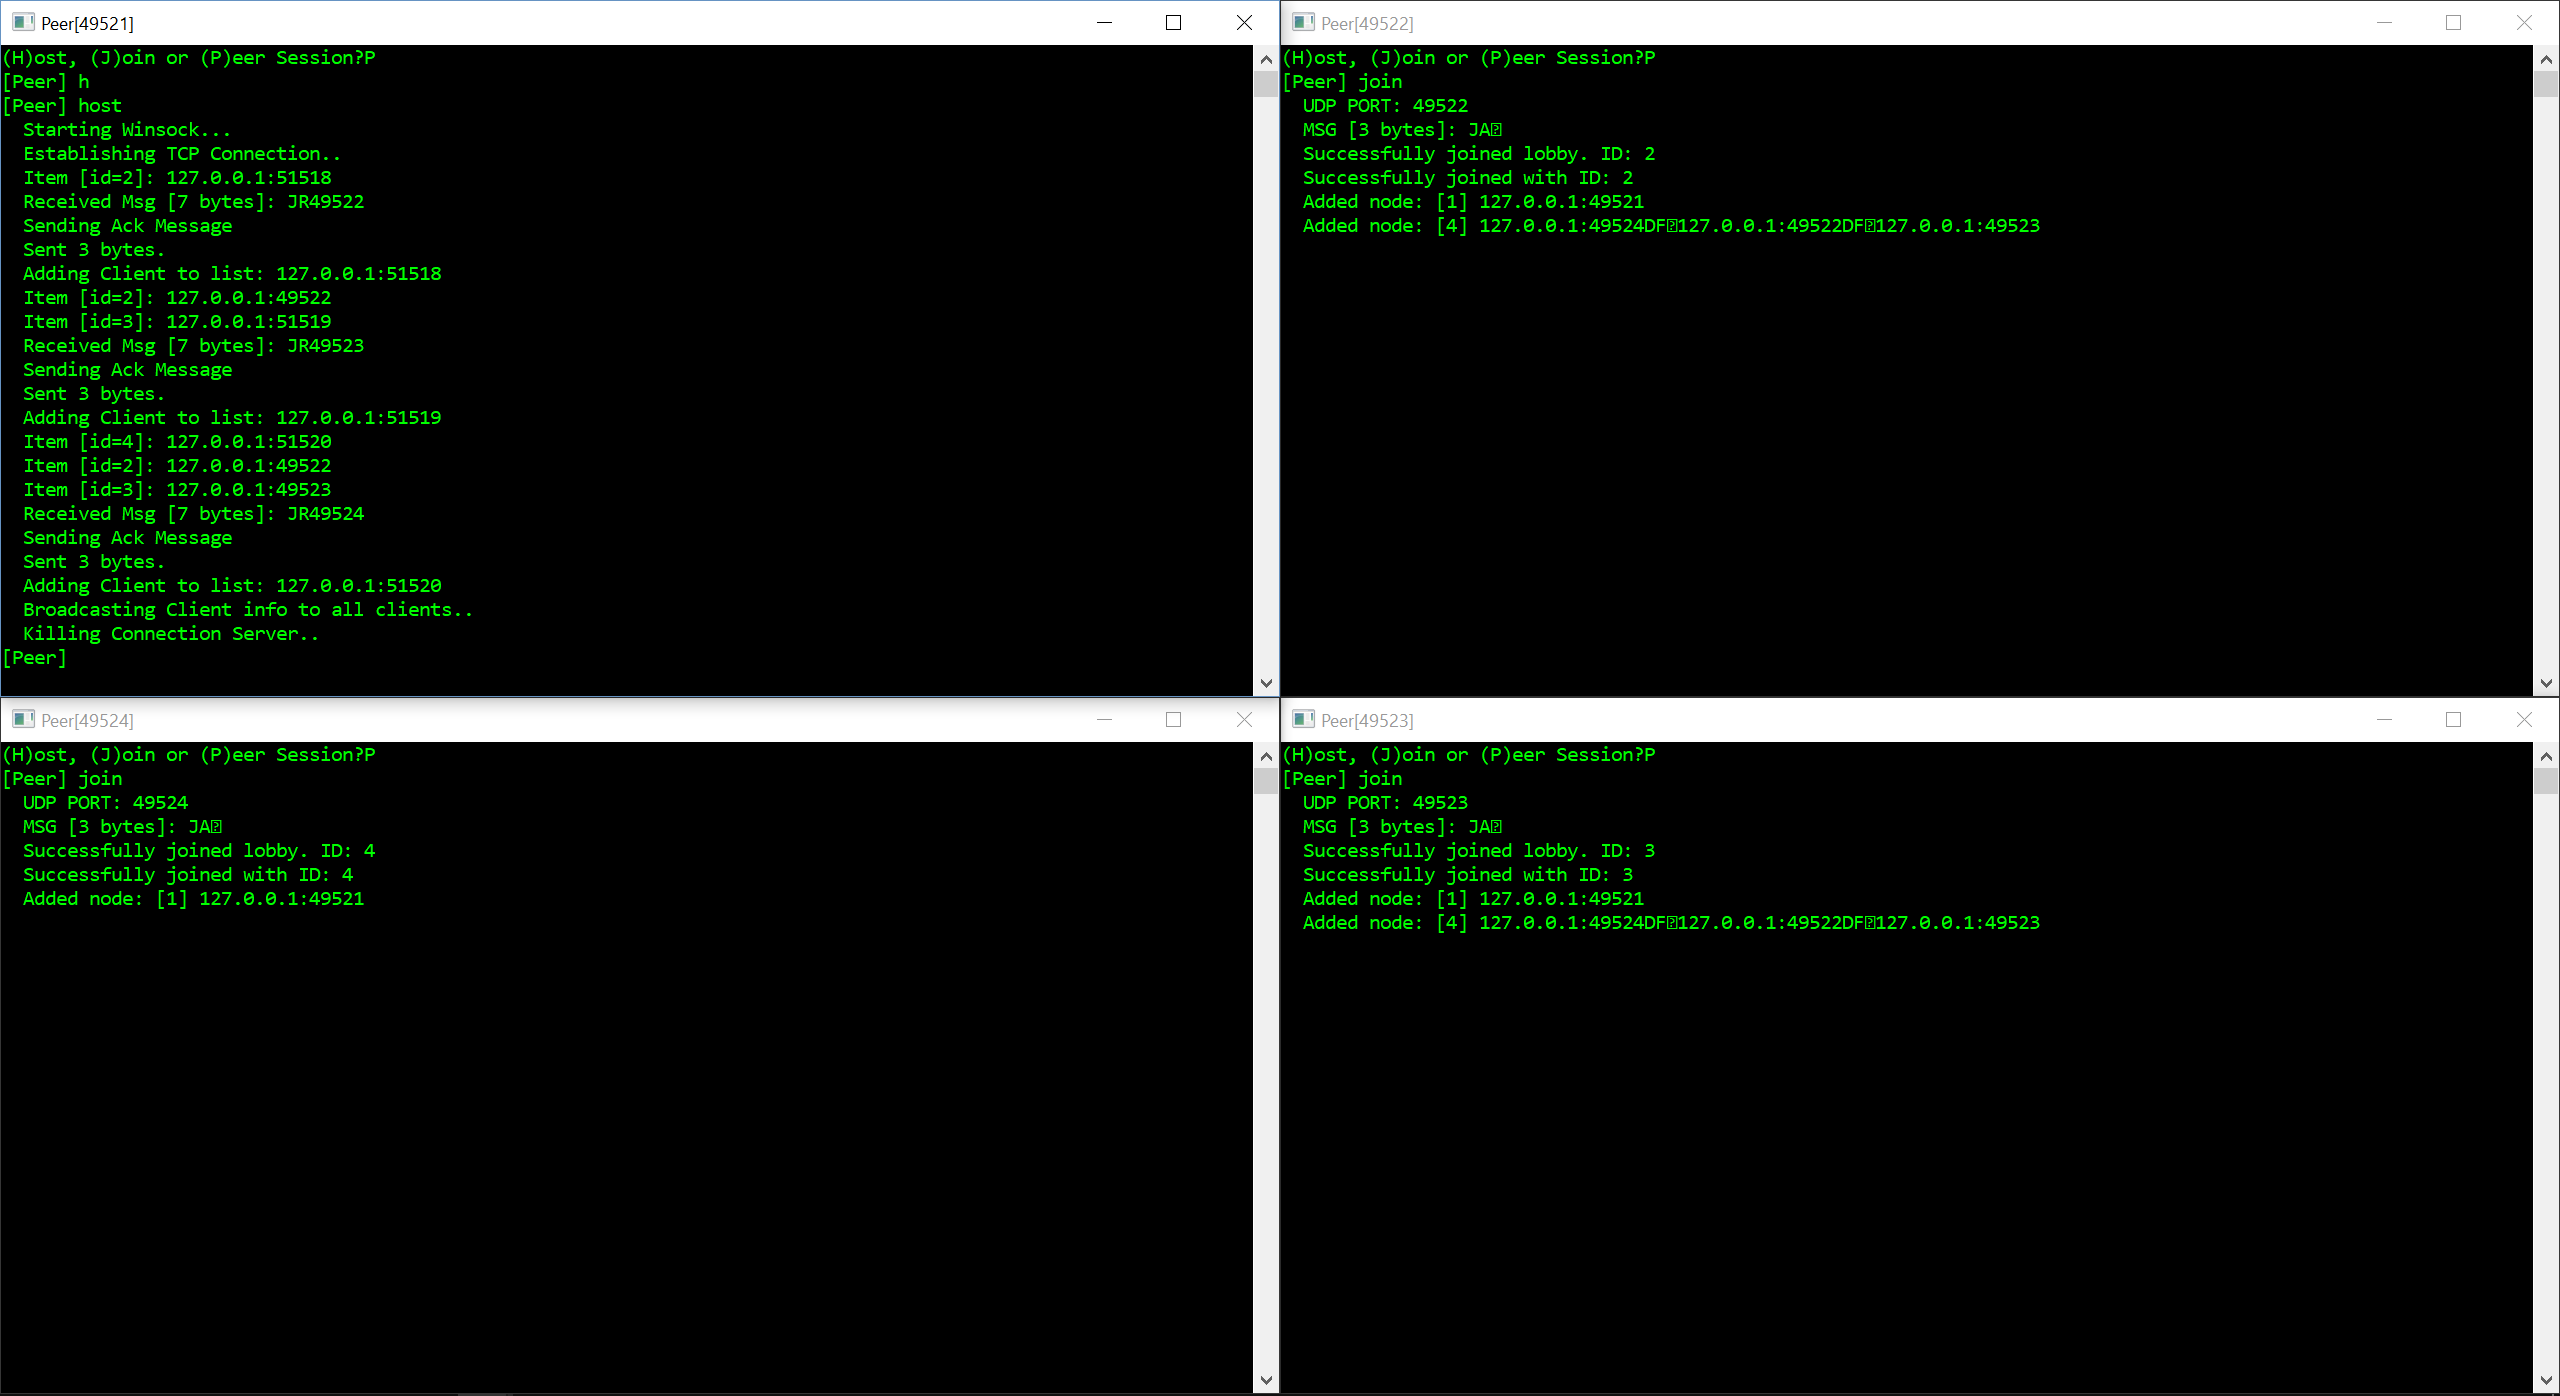
\includegraphics[width=\textwidth]{GNAT/sending_too_fast.png}
  \caption{Messages being broadcast with no delay}
  \label{fig:broadcast_too_fast}
\end{figure}

\begin{figure}[!h]
  \centering
  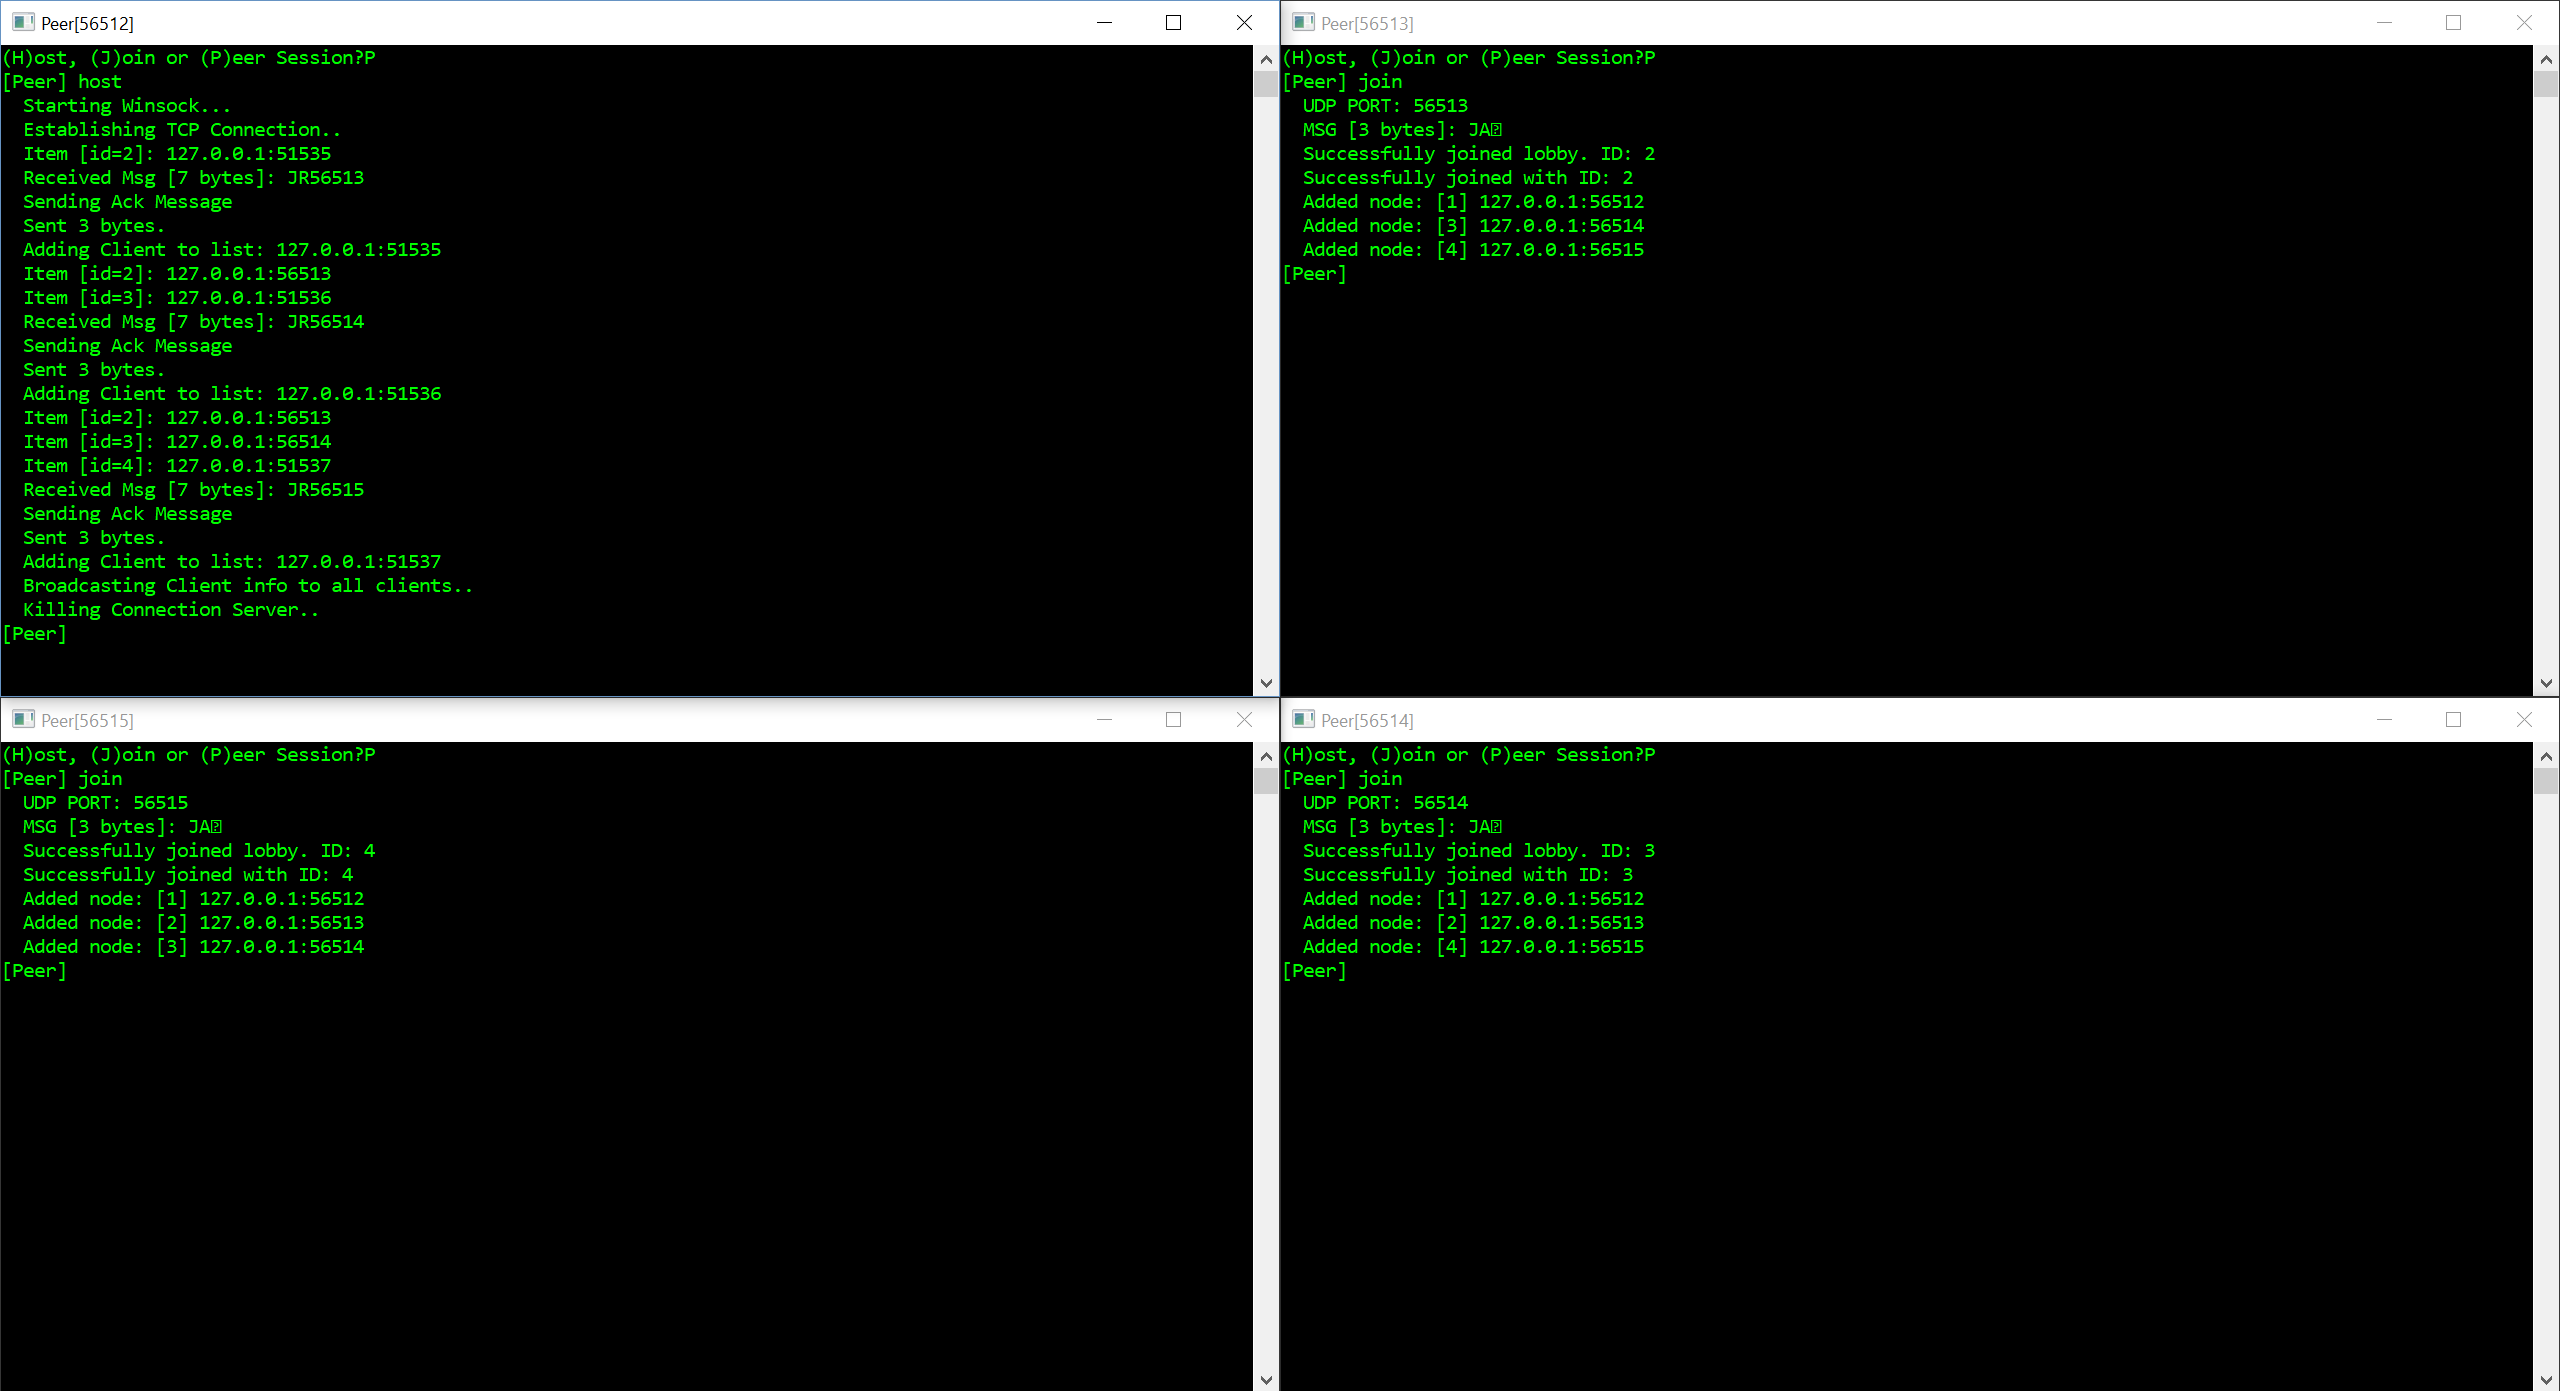
\includegraphics[width=\textwidth]{GNAT/sending_with_delay.png}
  \caption{Messages being broadcast with delay}
  \label{fig:broadcast_with_delay}
\end{figure}
\vfill
\newpage
